% !TEX TS-program = pdflatex
% !TEX encoding = UTF-8 Unicode

% Example of the Memoir class, an alternative to the default LaTeX classes such as article and book, with many added features built into the class itself.

%\documentclass[12pt,a4paper]{memoir} % for a long document
\documentclass[10pt,letterpaper]{memoir} % for a short document

\usepackage[utf8]{inputenc} % set input encoding to utf8

\usepackage{colortbl}
\usepackage[dvipsnames]{xcolor}
\usepackage{minted}
\usepackage[section]{placeins}
\usepackage{mdframed}
\usepackage{geometry} % to change the page dimensions
\geometry{letterpaper} % or letterpaper (US) or a5paper or....
\geometry{margin=0.75in} % for example, change the margins to 2 inches all round

% Don't forget to read the Memoir manual: memman.pdf

%%% Examples of Memoir customization
%%% enable, disable or adjust these as desired

%%% PAGE DIMENSIONS
% Set up the paper to be as close as possible to both A4 & letter:
%\settrimmedsize{11in}{210mm}{*} % letter = 11in tall; a4 = 210mm wide
%\setlength{\trimtop}{0pt}
%\setlength{\trimedge}{\stockwidth}
%\addtolength{\trimedge}{-\paperwidth}
%\settypeblocksize{*}{\lxvchars}{1.618} % we want to the text block to have golden proportionals
%\setulmargins{50pt}{*}{*} % 50pt upper margins
%\setlrmargins{*}{*}{1.618} % golden ratio again for left/right margins
%\setheaderspaces{*}{*}{1.618}
%\checkandfixthelayout 
% This is from memman.pdf

%%% \maketitle CUSTOMISATION
% For more than trivial changes, you may as well do it yourself in a titlepage environment
%\pretitle{\begin{center}\sffamily\huge\MakeUppercase}
\posttitle{\par\end{center}\vskip 0.5em}

%%% ToC (table of contents) APPEARANCE
\maxtocdepth{subsection} % include subsections
\renewcommand{\cftchapterpagefont}{}
\renewcommand{\cftchapterfont}{}     % no bold!

%%% HEADERS & FOOTERS
\pagestyle{ruled} % try also: empty , plain , headings , ruled , Ruled , companion

%%% CHAPTERS
\chapterstyle{hangnum} % try also: default , section , hangnum , companion , article, demo

%\renewcommand{\chaptitlefont}{\Huge\sffamily\raggedright} % set sans serif chapter title font
%\renewcommand{\chapnumfont}{\Huge\sffamily\raggedright} % set sans serif chapter number font

%%% SECTIONS
%\hangsecnum % hang the section numbers into the margin to match \chapterstyle{hangnum}
%\maxsecnumdepth{subsection} % number subsections

%\setsecheadstyle{\Large\sffamily\raggedright} % set sans serif section font
%\setsubsecheadstyle{\large\sffamily\raggedright} % set sans serif subsection font

%% END Memoir customization

\usepackage{bm}
\usepackage{graphicx}
\graphicspath{{./Images/}}
\usepackage{hyperref}
\hypersetup{
	colorlinks=true,
	linkcolor=blue,
	filecolor=magenta,      
	urlcolor=cyan,
}
\urlstyle{same}

\newcommand{\iic}[0]{$I^{2}C$}
\newcommand{\apiheader}[2]{\noindent{}\textbf{Header \emph{#1}}\\\noindent{}\textbf{Namespace: \emph{#2}}}

\title{Chandra Library User's Guide}
\author{Martin Jay McKee}
%\date{} % Delete this line to display the current date

\colorlet{binarybg}{SeaGreen!20!White!80!}
\colorlet{textbg}{Cyan!10!White!90!}
\newcolumntype{g}{>{\columncolor[gray]{0.95}}c}
\newcolumntype{B}{>{\columncolor{binarybg}}c}
\newcolumntype{T}{>{\columncolor{textbg}}c}

%%% BEGIN DOCUMENT
\begin{document}
%\begin{titlepage}
%\center{\Huge{Chandra Library User's Guide}}
%\end{titlepage}

\maketitle
\tableofcontents* % the asterisk means that the contents itself isn't put into the ToC

\chapter{Overview}
Chandra is a collection of almost entirely header-only libraries that are designed to support the development of real-time embedded control systems on microcontroller systems.  While Chandra supports running inside an RTOS, it does not require it nor is it specifically designed for such usage as the libraries are designed such that functionality can easily accessed from an explicit event loop.  There is a single ``core'' .cpp file that defines the whole Chandra runtime\footnote{Currently there is only a single variable definition which could also be defined directly in the application code.  In future, however, additional values could be defined and, as such, it is cleaner to place them in the .cpp file.}.  Chandra is best understood as not, strictly, a single library, but as a combination of libraries described in the following.  The goal of Chandra is to provide powerful and safe abstractions without using excessive resources either in storage or computation. 

\section{Description}
As they stand, the Chandra libraries consist of five sub-libraries: Chandra-Core, Chandra-HAL, Chandra-Interface, Chandra-Control, and Chandra-Aero.  The Chandra Core libraries are functionality that is required for any of the other libraries but which is - otherwise - stand alone.  The core libraries could be used completely by themselves, though they do not provide enough functionality to implement a complete application because they do not contain features such as input and output.  The HAL libraries provide a hardware abstraction layer for the platform with a consistent API.  This is the only sub-library that requires explicit porting to new processor platforms\footnote{In future, it may make sense to optimized some of the core functionality based on the platform.  This might include choosing loop variable sizes or other micro-optimizations.  The core functionality should work without requiring any porting, however.}.  The HAL includes things such as a system clock implementation, timing functionality, GPIO, serial peripherals, etc.  Some of the functionality in the HAL is platform independent as it is based directly on lower level functionality.  The porting documentation later in this guide describes what types and functions need to be implemented.  The third sub-library is Chandra-Interface which includes drivers for external components such as GPS, IMU, Baro, ADC/DAC, pin expansion, etc.  The drivers are platform independent and depend upon Chandra-HAL.  Forth thre is Chandra-Control which provides observers, filters and control loop implementations.  Finally, Chandra-Aero provides special-purpose functions for aerodynamics related programs.  This includes functionality such as an atmosphere (~altitude, pressure, temperature, density~) model, basic air properties, lift and drag calculation, etc.

\section{Dependencies}
The Chandra libraries are written against the C++14 standard and require a compiler which is compatible with the standard, including language features such as: ranged for loops, generalized lambda expressions, constexpr expressions, and variadic templates.  Any C++14 compliant compiler should have no issues with the code.  Only minimal standard library support is needed but includes: chrono, type\_traits, number\_traits, and std::common\_type.  

To use the code generators bundled with Chandra, it is also necessary to have a Python 3 interpreter installed along with several libraries.  To run the generator for Chandra Units, the Mako Templating engine is required.  For the Kalman Filter Optimizer, Mako and SymPy are required.

The documentation is built in LaTex and requires a number of packages including pygments (~which - in return - requires Python~) and graphicx.  In general, users should not need to rebuild the documentation as Chandra is distributed with the final built PDF of the documentation.
 
\section{Platform Independence}
The bulk of the Chandra libraries are platform independent.  The only portion of the libraries which are platform dependent are those within Chandra-HAL -- the \emph{H}ardware \emph{A}bstraction \emph{L}ayer.  Porting of the HAL functionality to new platforms is required but the remainder of the libraries can be used with no changes so long as a C++14 compiler and standard library are available.  If some standard library features are unavailable on the target platform, they can also be included externally.

\section{User's Guide Organization}
This guide is arranged in five major sections.  The first, this overview, is simply a high-level overview which should be sufficient for a new user to understand what the Chandra library is - in a basic way - but ability to use the library should not be expected by this point.  The following four sections are intended to provide a deeper introduction to the components in the library, as well as rationale, usage information, and general reference.  The second section of the guide is a getting started chapter which includes ?? complete applications (~targeted at an NXP LPCXpresso845MAX development board) to demonstrate basic use of the library, features, code structure, and compilation.  The third section of this guide covers the overall library architecture.  It introduces all the major components of the library and the rationale for including them.  Following the architecture documentation, the is an in depth API (~\emph{A}pplication \emph{P}rogrammer \emph{I}nterface~) reference which describes the complete interface for every type and function.  The final section of the guide is a code ``cookbook'' which includes code fragments to solve specific problems\footnote{Unless otherwise specified, the cookbook code is platform independent.}.  This final section is intended to simplify the learning of the library as well as demonstrating some of the less obvious features.

Beyond the primary descriptive sections there are appendicies which include generally useful information that does not fit in the aforementioned sections.  These subjects include how to set up the default development environment for the NXP processors, a guide on the process of porting the platform specific portions (Chandra-HAL) of the library, as well as general notes on functionality that go beyond what is required for a general understanding of the library.  At the end there is a list of the references mentioned throughout the guide.

\part{Library Introduction}
\chapter{Getting Started}
The Chandra libraries were originally written for personal projects targeting the NXP LPC series of ARM Cortex-M microcontrollers.  Despite this, however, the Chandra libraries were written from the very beginning to expose an interface that can be ported to multiple architectures without loss of functionality.  The Chandra libraries are designed to be extremely powerful without being too excessively difficult to use.  Furthermore, they are designed with safety in mind.  While they may not be as simple to use as an Arduino compatible platform, the libraries are designed in such a way as to provide more direct access to the hardware and so that they can be optimized\footnote{Compilation of an application built on the Chandra Libraries without compiler optimization \emph{WILL} lead to large slow programs.  Chandra is implemented using templates and other C++ features that cause bloated unoptimized code.  Nevertheless, when compiler optimization is enabled, much of the functionality is optimized to very nearly the hand-written equivalent.  Do not compile Chandra programs without optimization and expect svelte code.  You won't get it.  With optimization, however, you will.} to a much higher level than some of the core Arduino functionality.  Having said that, Chandra is not a competitor to Arduino.  It is aimed at implementing control systems.  Specifically, it is designed for things like rovers and flight computers.  Additionally, while it could certainly be used for high-level systems, it is mostly intended for deeply embedded, real-time systems.

This section will introduce some of the central concepts and functions in the Chandra library in the context of example applications.  

\section{An Embedded Hello World}
As is typical of embedded (microcontroller) platforms, the first introduction to code will blink a single LED (~\emph{L}ight \emph{E}mitting \emph{D}iode~).  For those used to the basic blink of Arduino, however, the code may look unusual due to the fact that Chandra is intended to be used in an event-driven manner.  The whole blink code is as follows.
\begin{minted}[linenos]{cpp}
// Standard Includes
#include <chrono> // std::chrono
using namespace std::literals::chrono_literals; // Use chrono UDL suffixes

// Chandra Includes
#include<chrono.h> // Chandra-Core clock functions
#include<leds.h> // LED object definitions

chandra::io::LED led(0, 0, true); // Construct the LED object

int main(void){
	chandra::chrono::timestamp_clock::init(); // Initialze the processor clock

	led.breathe(1s); // Configure the LED to breathe over 1 second
	
	while(true) {
		led.update(); // Update the LED as needed
	}
	
	return 0;
}
\end{minted}
There are four lines in the code that are implementing the functionality.  On line 9 the LED object (\emph{led}) is created -- passing in the port and bit number of the GPIO pin.  This line is platform dependent as some ports (such as the Arduino port) may use a different method of identifying the pin to use.  On the default platform \footnote{NXP LPCxpresso845Max development board}, the green LED is connected on port 0, bit 0.  The final parameter (\emph{true}), specifies that the LED is connected in an active-low configuration.  Regardless of the configuration, the LED is initialized in the off state.  The second functional line is line 12 which calls the built-in processor clock initialization function.  This function hides all the platform specific code for generating a continuous timestamp clock.  It is not only platform dependent but may also function differently based on preprocessor directives.  These directives are outlined in the library deep-dive portion of this manual.  In any case, this line should be the first line of any Chandra based program to ensure that the clock is running and initialized.  In so doing, timed functions (such as the LED blink here) will work correctly, but other portions of the library depend upon the clock rate having been calculated.

Line 14 tells the LED object that the function it is to perform is to breathe (increase and decrease in brightness) with a period of one second.  Chandra uses the C++ standard library std::chrono to define time periods and here the user defined literal from chrono \emph{1s}, to cleanly specify 1 second.  At this first call to the \emph{breathe()} function, the LED will update its state when its \emph{update()} method is called.  This happens in an infinite loop on line 17, leading to an LED that breathes indefinitely.

While this example demonstrates the creation of the hardware objects and all includes in a single file, it is better form with Chandra to move such hardware into external \emph{hw.h}/\emph{hw.cpp} files.  In this case, the modified source would look something like the following.  First \emph{hw.h} would contain,
\begin{minted}[linenos]{cpp}
#ifndef HW_H
#define HW_H
#include<leds.h> // LED object definitions

extern chandra::io::LED led; // Define the LED object
#endif
\end{minted}
the \emph{hw.cpp} file,
\begin{minted}[linenos]{cpp}
#include "hw.h"
chandra::io::LED led(0, 0, true); // Construct the LED object
\end{minted}
and the \emph{main.cpp} file,
\begin{minted}[linenos]{cpp}
// Standard Includes
#include <chrono> // std::chrono
using namespace std::literals::chrono_literals; // Use chrono UDL suffixes

// Chandra Includes
#include<chrono.h> // Chandra-Core clock functions

#include "hw.h"

int main(void){
	chandra::chrono::timestamp_clock::init(); // Initialze the processor clock
	
	led.breathe(1s); // Configure the LED to breathe over 1 second
	
	while(true) {
		led.update(); // Update the LED as needed
	}
	
	return 0;
}
\end{minted}
Due to its simplicity, there is little savings in the application file in this case.  In more complicated programs, however, the hardware files can absorb quite a bit of variable creation boilerplate and this general structure leads to clearer application code.


\chapter{Library Architecture}
\section{Overview}
The following sections provide an outline of the library facilities.  Each feature will be explained and a very basic example of use provided.  Complete description of the API is saved for the API chapter which is arranged in a manner that mirrors this chapter.  Essentially, this chapter is an introduction to functionality and the rationale behind it while the API reference gets into the nuts and bolts of each function, class, and datatype provided by the library.

\section{Core}
\subsection{Math}
\subsubsection{Matrix Types}
The 
ADD SYMMETRIC AND SKEW-SYMMETRIC MATRICIES.  THESE CAN HAVE OPTIMIZED STORAGE AND MAY BE POSSIBLE TO OPTIMIZE OPERATIONS FOR THESE SPECIFIC FORMS (I.E. ADDITION CAN BE OPTIMIZED, MULTIPLICATION THAT CREATES A SKEW-SYMMETRIC MATRICIES MAY BE OPTIMIZABLE, ETC.

\subsubsection{Matrix Operations}
IT MAY MAKE SENSE TO USE EXPRESSION TEMPLATES TO SELECT THE IMPLEMENTATION OF OPERATIONS.

\subsubsection{Matrix Views}
NEED TO MAKE SURE THAT THE MATRIX VIEWS ARE WORKING AS I WANT THEM TO AND THAT THEY ARE USED THROUGH THE DRIVERS WHERE APPROPRIATE.

\subsection{Units}

\section{HAL}
\subsection{Chandra::Chrono}
\subsubsection{System Clock}
To configure the timestamp clock, a preprocessor directive describing the onboard peripheral that will be used as the source is used. \\
	\begin{centering}
	\begin{tabular}{cgc}
		\rowcolor[gray]{0.8}\textbf{Preprocessor Symbol}  & \textbf{Definition}\\
		SCT\_HARDWARE\_TIMESTAMP\_MODE & Use an SCT clock as the timestamp generator\\
		SYSTICK\_SOFTWARE\_TIMESTAMP\_MODE & Use the SysTick clock as the timestamp generator\\
		
	\end{tabular}
	\end{centering}

\subsubsection{System Frequencies}
\subsubsection{Performance Timers}

\subsection{General Purpose Input/Output}
\subsection{Analog Input/Output}
CURRENTLY THERE IS NO API SPECIFIED FOR DAC, THERE SHOULD BE.

\subsection{Communications}
\subsubsection{\iic}
\subsubsection{SPI}
\subsubsection{USART}

\section{Interface}
\subsection{Drivers}
\subsubsection{Analog Input/Output}
THESE ARE DRIVERS FOR EXTERNAL ADCS AND DACS.  THE API IS THE SAME AS THE INTERNAL ADC/DAC INTERFACE BUT THESE DRIVERS ARE PLATFORM INDEPENDENT BECAUSE THEY DEPEND UPON THE COMMUNICATION SUPPORT IN THE HAL.
\subsubsection{GPS}
NEED TO COME UP WITH AN API AND A COMPUTATIONAL ENGINE TO BASE ALL OF THE DRIVERS ON.
\subsubsection{Inertia Measurement Sensors}
\subsubsection{Servo Drivers}
\subsubsection{RF Transceivers}
CURRENTLY THIS ONLY HAS THE RFM9X

\section{Control}
\subsection{Kalman Filtering}
The Kalman filtering components of the Chandra library are designed to support multiple approaches to constructing a kalman filter.  Explicit implementation of a Kalman filter directly in source code by configuring the various matricies is simple.  This also has the advantage that it allows for dynamic modification of the matricies during runtime.  A second method for constructing a kalman filter for Chandra projects is to use the included code generator.  This generator takes as input a description file which includes descriptions of variables and the state as well as the state transition and measurement equations; and it constructs the required code C++ for the Kalman filter.  This constructed filter provides the exact same API as the built-in explicit kalman filter.  Additionally, it will do simplification of the resultant equations to minimize the computational load of the final filter.  Currently, the code generator only works 

\subsubsection{Code Generator}
The code generator is written in the Python programming language and uses the SymPy library to handle symbolic representations of the Kalman equations.  This is how it is able to do operation reduction (subexpression folding) as well as pre-calcuation of constants and multiplication by unity and zero.  The code generator currently only works with the basic Kalman Filter formulation but is intended to be expanded to also work with -- at least -- the Extended Kalman Filter (EKF) and Unscented Kalman Filter (UKF).  In so doing, the code generator should speed the implementation and testing of various algorithms in Chandra applications.

\subsection{PID}

\subsection{Static IMU Calibration}
The basic IMU calibration API is based on the structure found in NXP application note AN4399.  This white paper -- which discusses high-precision, full 12 parameter calibration of accelerometers -- looks at various optimal measurement orientations for calibration of accelerometer offsets and gains in addition to formulating a least means squared approach to calculating the calibration parameters.  The API\footnote{\emph{A}pplication \emph{P}rogrammer \emph{I}nterface} provides calibration objects for accelerometer only, gyroscope only, magnetometer only, accelerometer/gyroscope, accelerometer/magnetometer, and 9-axis sensors.  The calibration completed is limited to a static calibration and, as such, it does not provide the information required to calibrate gyroscope gains.  It does, however, provide sufficient information for an initial gyro bias calibration.  All of these objects follow the same general API where a calibration is started and for each step the required orientation of the sensor is returned.  This allows for a manual repositioning of the IMU prior to the next measurement.  When the required number of steps have been completed, the calibration values are calculated, the IMU object -- optionally -- updated, and the calibration is complete.

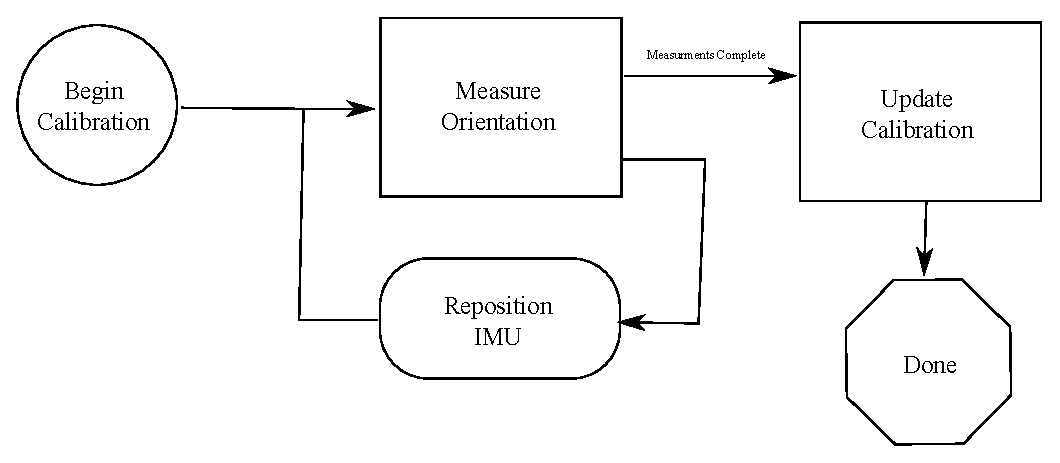
\includegraphics{imu_calibration_flow.eps}

The default measurements provided by the IMU calibration as defined in the aforementioned application are -- generally -- insufficient to do a complete calibration of a magnetometer and thus the built-in static calibration objects do not include a full calibration of the magnetometer.  Basically, the most that can be done with the current API is a 12-parameter calibration of the accelerometers, a 3-parameter (bias-only) calibration of the gyroscopes, and a low-resolution 6-parameter calibration of the magnetometers (axis scale and bias).  Dynamic calibration is required to calibrate the gain parameters of the gyroscopes while a greater number of samples are required to calculate an accurate ellipsoidal fit for the magnetometer calibration.

Given an IMU object named \emph{imu}, the following code demonstrates the calibration procedure.
\begin{minted}[linenos]{cpp}
// Create the calibrator object with default parameters (orthagonal cubic calibration)
auto imu_calibrator = StaticIMUCalibrator<>(imu);
auto cal_start_result = imu_calibrator.init();
// ... reposition to cal_start_result.next_orientation
bool done = false;
while(!done) {
	// Take a measurement step at the default orientation
	auto cal_step_result = imu_calibrator.measure();
	done = cal_step_result.complete;
	// ... reposition to cal_step_result.next_orientation
}

// Calculate the calibration and apply to the IMU
auto cal_final_result = imu_calibrator.calibrate();
\end{minted} 
While the simplest possible version, this code does -- at least -- introduce the general usage of the static calibrator objects.  There are three functional calls: \emph{init()}, \emph{measure()}, and \emph{calibrate()}.  Each of these return an object which contains data useful for the tracking and control of the calibration process.  

By default the call to \emph{calibrate()} will update the calibration in the passed in \emph{imu} object.  The calibration parameters will be calculated regardless and returned as members of the return value.  Passing \emph{false} to this function will disable the update of the calibration but still return the parameters.

The StaticIMUCalibrator object has member functions which access the parameters of the calibration such as number of measurement orientations, the target orientations, the number of samples to take for each measurement, the type of calibration (3-/6-/12- parameter) of each sensor, etc.  Information regarding the complete API is contained in the Library Deep Dive section while there is an appendix containing general notes on IMU calibration in general.

\subsection{Builtin Estimators}
\subsubsection{Madgwick's AHRS}
\subsubsection{Alpha-Beta-(Gamma)-(Eta)}

\section{Aero}
ATMOSPHERIC PROPERTIES, MODEL OF ATMOSPHERE (PRESSURE, DENSITY, TEMPERATURE, ALTITUDE, ETC.), BASIC AERODYNAMICS
\subsection{Atmosphere Calculations}
\subsection{Gravity Calculations}
The gravity library provides calculation of surface and airborne gravity calculations to moderate accuracy.  Both magnitude of effective gravity and vector results are available, depending upon configuration.  The library provides a single class \mintinline{cpp}{Gravity<>} which is a highly configurable object that takes a number of compile-time arguments to determine the gravity model being used, the corrections applied, and if a vector value is desired.  To account for simple usages, three aliases are also defined: \mintinline{cpp}{StandardGravity<>}, \mintinline{cpp}{StandardGravity<>}, and \mintinline{cpp}{StandardGravity<>}.  These aliases of the gravity class provide both the lower precision, low-cost options and the highest-accuracy options.  As such, they should be sufficient for most usages.  Of course, Section \ref{sec::gravity:calculation::api} of this manual (in the API reference) provides information about all the features of the gravity object, . 

Three models of gravity are available: a constant standard gravity, the 1980 IGF (Internaltional Gravity Formula), and WGS84 (\emph{W}orld \emph{G}ravity \emph{S}urvey).  The constant gravity model is intended for low-accuracy, performance and memory critical applications and just returns the international standard gravity value of $9.80665 ms^{-2}$.  The IGF and WGS84 approximations are much more accurate but have higher system requirements.

The corrections available are two free-air correction approximations, a slab correction, and a centripetal correction.  Each of these corrections can be applied or ignored.  Generally they are fairly small corrections and, as such, ignoring them is reasonable in the case of a constrained system.  The low-precision approximation of the free-air correction, however, only costs a single multiplication and so should generally be included in all cases that airborne gravity estimates are needed.

The gravity calculations are cross-checked and also compared to the values generated by the calculator at: \url{http://walter.bislins.ch/bloge/index.asp?page=Earth+Gravity+Calculator}.  It should be noted that the gravity vectors returned on this webpage are in ECEF (\emph{E}arth \emph{C}entered-\emph{E}arth \emph{F}ixed) coordinates.  The examples in this documentation, on the other hand, use a local tangent NEU (\emph{N}orth-\emph{E}ast-\emph{U}p) coordinate system.  The gravity object is also able to return vectors in ECEF coordinates if desired.

\part{Library API}
\chapter{Math}
\section{Linear Algebra}
\section{Quaternions}
\section{Rotations}
\section{Math Utilities}

\chapter{Units}

\chapter{Chrono}
\section{System Frequencies}
\section{Timestamp Clock}
\section{Conversions between std::chrono and chandra::units}
NONE.  THIS DOESN'T HAPPEN, AT THE MOMENT.  IT REALLY SHOULD THOUGH.

\chapter{General Purpose Input/Output}

\chapter{Analog Input/Output}

\chapter{Communications}
\section{\iic}
\section{SPI}
\section{USART}

\chapter{Drivers}
\section{External Analog Input/Output Drivers}
\section{Temperature Sensor Drivers}
\section{Pressure Sensor Drivers}
\section{Inertial Motion Sensor Drivers}

\chapter{Control}
\section{Recursive Filters}
\section{Alpha-Beta-(Gamma)-(Eta) Filtering}
\section{Kalman Filtering}
\section{PID Control}
\section{Static IMU Calibration}

\chapter{Aero}
\section{Atmospheric Calculations -- \mintinline{cpp}{class Atmosphere<>}}
\label{sec::atmosphere:calculation::api}
\apiheader{atmosphere.h}{chandra::aero}
\subsection{Class Template Arguments}
\subsection{Type Aliases}
\subsection{Constructors}
\subsection{Accessors}

\section{Gravity Calculations -- \mintinline{cpp}{class Gravity<>}}
\label{sec::gravity:calculation::api}
\apiheader{gravity.h}{chandra::aero}
\subsection{Class Template Arguments}
\begin{minted}{cpp}
template<
	class Value,
	GeoidCoordinates VectorCoordinates = None,
	uint32_t Flags = ApproxFreeAirCorrect,
	class AngleUnits = rad,
	class LengthUnits = m,
	class AccelerationUnits = m_per_s2
>
class Gravity;	
\end{minted}
The gravity class has six compile-time arguments, with the last five defaulted.  The first argument, \mintinline{cpp}{Value}, is the value type to be used.  For full accuracy of the WGS84 model, this should be either \mintinline{cpp}{double} or \mintinline{cpp}{long double}, but it can be \mintinline{cpp}{float} for less demanding applications or even user-defined types \footnote{The \textbf{Iamb}, fixed-point types will work as a type, though they require special implementations of the models and are less accurate.}.  

The second argument, \mintinline{cpp}{VectorCoordinates}, is currently limited to \emph{None}, \emph{ECEF}, or \emph{NEU} with \emph{None} being the default.  If the vector coordinates are \emph{None}, the constructed gravity object will not even include the vector accessor methods and the additional code to generate vectors will not be included.  The code is added when a valid form of coordinates are selected.  In addition to defaulting to magnitude only mode in the class itself, the aliases function in the same way -- defaulting to magnitude only but allowing the passing of coordinates to \emph{turn on} vector support.  These valid coordinates are defined in the \emph{GeoidCoordinates} enumeration found in the \emph{geoid.h} header.

The third argument, \mintinline{cpp}{Flags}, is an integer that contains all the implemented features such as the gravity model and enabled corrections.  These flag values are public static members of the \mintinline{cpp}{GravityConfig} class, also in the \mintinline{cpp}{chandra::aero} namespace of the \emph{gravity.h} header.   

TALK ABOUT THE FEATURES AND WHAT THE VALID FLAGS.

\subsection{Type Aliases}

\subsection{Constructors}

\subsection{Accessors}



\part{Chandra Cookbook}
\chapter{Clock and Timing}
\section{Performance Timers}
\subsection{Timing a function}
\subsection{Conditional timing of a function}
\subsection{Loop frequency measurement}
\subsection{Loop frequency statistics}

\chapter{Digital I/O}
\section{Reading a digital pin}
\section{Writing to a digital pin}
\section{Reading a mechanical switch/button}
\section{Manual control of an LED}
\section{Automatic PWM of an LED}
\section{Automatic PWM of an LED with asynchronous update}
\section{Event on a pin falling (rising) edge}
\section{Reading a Quadrature Encoder}

\chapter{Analog I/O}
\section{Raw reading of a single ADC channel}
\section{Scaled reading of a single ADC channel}
\section{Reading multiple ADC channels}

\chapter{Math}
\section{Conuct a matrix}
\section{Solve a system of equations}
\section{Invert a matrix}

\chapter{Control}
\section{Kalman}
\section{PID}
\section{IMU Calibration}

\chapter{Aero}
\section{Atmosphere}
\subsection{Pressure and density at a known altitude}
\subsection{Altitude from pressure}
TODO: do both in standard conditions and in non-standard conditions.

\section{Gravity}
\subsection{Acceleration due to gravity on the Earth's surface}
\subsection{Gravitational acceleration above Earth's surface}

\appendix
\part{Appendicies}

\chapter{Setting up MCUXpresso for LPC Series Microcontrollers}
\section{Installation}
\section{Optimization and Standards}
\section{Include Paths}
\section{Preprocessor Definitions}

\chapter{Porting Guide}
The only section of the Chandra libraries that require porting when moving to new platforms is the Chandra-HAL components.  Any other components (core, control, and aero) are platform independent.

ALL COMPONENTS THAT REQUIRE PORTING NEED TO HAVE HEADER TEMPLATES.
\section{Low-Level Register Access}
THIS IS THINGS LIKE CLOCK POWER, PERIPHERAL RESET, GPIO MAPPING, ETC.
\section{Clock and Frequencies}
\section{GPIO}
\section{ADC}
\section{Timers}
THERE IS NO TIMER API DEFINED AT THE MOMENT, BUT THERE REALLY SHOULD BE ONE...
\section{\iic}
\section{SPI}
\section{USART}

\section{(Optional) DAC}
\section{(Optional) Special Peripherals}

\chapter{Notes on IMU Calibration and Errors}
IMU sensors -- including accelerometers, gyroscopes, and magnetometers -- present a wide range of potential error sources.  The drivers contained in Chandra include the equations for a full twelve-parameter calibration which will correct for the most basic static errors.  Even so, there are a number of dynamic effects that the built-in calibration is unable to correct.  Both of these effects are outlined here.

\section{Static Calibration}
The static calibration of an IMU sensor is defined by the following general equation.
\begin{equation}
	\vec{y_c} = \mathbf{W}\vec{y_m} + \vec{b}
\end{equation}
Here the quantity measured from the sensor is $\vec{y_m}$, $\vec{b}$ is a bias value, and $\mathbf{W}$ is a gain matrix.  The calibrated value $\vec{y_c}$ is the result.  This general form hides several possible sources of error which may be calibrated out.  The bias is the least complicated.

Bias is a -- generally -- constant offset from the value the sensor should be measuring.  As long as the bias is small, it may not cause massive issues for accelerometers or magnetometers when used for orientation estimation.  If small, the bias only causes a small error in the calculated orientation.  When accelerometers are used for inertial navigation or gyroscopes for orientation tracking, however, the bias term becomes especially important as the sensor readings are integrated.  This integration causes the bias term to effect the estimation without bound.  As such, for AHRS and MARG applications it is vitally important that the gyroscope bias be corrected.  For INS applications, the accelerometer bias, also, needs to be corrected.

The gain matrix hides much more complexity than the bias; but it is no more difficult to understand.  Simply, the gain matrix can be represented as a combination of matricies which apply different transformations to the values.  These transformations may be bulk, such as physical rotation of the sensor represented by a matrix, $\mathbf{R}$, or corrective such as the axis scaling factor in a diagonal matrix $\mathbf{S}$.  Additionally, there are errors that result from the sensor axes being non-orthogonal or general misalignment (either in the package or on the board) which are represented by a matrix $\mathbf{O}$.  The final gain matrix then has the form,
\begin{equation}
	\mathbf{W} = \mathbf{R}(\mathbf{S}+\mathbf{O})
\end{equation}
Given that $\mathbf{R}$ is a known quantity for a particular PCB design, it is not included in the calibration but, rather, applied separately.  As such, when Chandra calculates gain calibration, it is calculating $(\mathbf{S}+\mathbf{O})$.  To do so, however, a correct value of $\mathbf{R}$ must be provided.  This is because the full $\mathbf{W}$ matrix is calculated and the calibration correction is then backed out by calculating,
\begin{equation}
	(\mathbf{S}+\mathbf{O}) = \mathbf{R^{-1}}\mathbf{W}
\end{equation}


\section{Dynamic Errors}
Unfortunately, neither bias nor gain error are truly static errors.  They may change with time and often change with temperature.  As such, any calibration that is completed is nothing more than an estimate.  Dynamic errors include things like temperature effects and noise.  

Some temperature effects cause a proportional change in the gain and/or bias of a sensors, in these cases the error can be calibrated out using gain matrix and bias vector corrected by a polynomial fit with temperature as the controlling parameter.  For instance, a two-temperature calibration may be corrected by using the following,
\begin{equation}
	\vec{b}(T) = \frac{(\vec{b_2}-\vec{b_1})}{(T_2-T_1)}(T - T_1) + \vec{b_1}
\end{equation} 
and,
\begin{equation}
	\mathbf{W}(T) = \frac{(\mathbf{W_2}-\mathbf{W_1})}{(T_2-T_1)}(T - T_1) + \mathbf{W_1}
\end{equation} 
Similar solutions may be found for a fit of any order $N$ so long as at least $N+1$ calibrations are calculated at different temperatures.  This temperature compensation, however, is not implemented as a core feature of the Chandra libraries due to it being highly application dependent.

Beyond the temperature effects that are possible to calibrate out, however, there are other error sources which cannot be handled so simply.  For instance, they may have the effect of superimposing a random walk error on the output.  This is often the case for rate gyro sensors.  When this happens, there is no consistent proportionality between the state of the sensor and the error of the measurement and, as such, it cannot be removed formulaically.  The only recourse is to use an adaptive filter such as a Kalman filter to both identify the error component and remove it.  As before, this is not directly implemented in the Chandra libraries being even more application dependent than temperature calibration.

Finally, sensors produce random noise.  This may be the result of electrical noise, and affect the magnitude of the measurement signal, or it may be a result of clock inaccuracy or clock jitter and affect the timing of a measurement.  Generally speaking, the only control that might be held over the electrical noise is to control the temperature of the sensor or the cleanliness of the power rails.  When running a calibration, Chandra will take multiple measurements at each orientation and generate an estimate of the standard deviation of the measurements which are an estimate of the random noise power.  This may be used to construct the noise covariance matrix for a Kalman filter or for other similar uses.  As with the gain and bias, the sampling clock rate may have a temperature dependence, but it is often not controllable in any meaningful way by the user.  On the other hand, some more advanced IMU sensors have the ability to return a timestamp value with a measurement or even run from an external clock.  To take advantage of this additional information, the Chandra drivers provide access to a measurement timestamp and sample period.  For sensors that do not provide a hardware timestamp, these are generated by the main processor.  If available, however, they are sourced from the sensor and corrected using the main clock as a reference.  This allows for the removal of clock inaccuracy so long as the main processor clock is more accurate.


\section{Modified Calibration Forms}
There are a couple of possible modifications to the calculation of the calibration which may be used internally to an IMU driver.  These are, primarily intended to reduce the computational complexity of generating the corrected value $\vec{y_c}$.  They may be used individually or in combination though not all combinations are valid or implemented in any particular driver.'


   
\subsection{Three-Parameter (bias only) or Six-Parameter Calibration}
If the IMU axes are known to be physically aligned with the body frame to be sensed, the rotation matrix $\mathbf{R}$ will be the identity matrix and some reduced complexity calibration options become reasonable to consider.  Firstly, the assumption that the sensor is perfectly aligned and orthogonal may be made and that reduces the calibration to six parameters.  Secondly, it may be assumed that three is no gain error whatsoever which will reduce the calibration to three parameters.  It should be understood, however, that due to the caching of calculating the matrix $\mathbf{W}$, these methods of calibration only reduce complexity in the case where it can be ensured that $\mathbf{R} = \mathbf{I}$.  If configured for three or six parameter calibration, the IMU driver loses the ability to set a rotation matrix and will cause a compile-time error if it is attempted.

By assuming perfect sensor alignment and orthogonality, the $\mathbf{O}$ matrix becomes zero so that the calibration equations become,
\begin{equation}
	\vec{y_c} = \mathbf{S}\vec{y_m} + \vec{b}
\end{equation}
Because $\mathbf{S}$ is a diagonal matrix, this reduces the number of multiplications required substantially and speeds up the calculation of $\vec{y_c}$.

Similarly, when doing a static calibration on a rate gyro sensor, there is no information available on the sensor magnitude accuracy.  As such, the only reasonable value for the scale matrix, $\mathbf{S}$ is the identity matrix and for $\mathbf{O}$ is the zero matrix.  That results in the calibration equations reducing to,
\begin{equation}
\vec{y_c} = \vec{y_m} + \vec{b}
\end{equation}
and requiring only additions.


\subsection{Hardware Sensor Bias}
The general form of the gain/bias calibration as described above is used for most sensors.  There are, however, some sensors which include internal offset calibration registers and that, therefore, remove the necessity to calculate the gain correction in the processor code.  In this case, the calibration may be calculated as,
\begin{equation}
	\vec{y_c} = \mathbf{W}\vec{y_b}
\end{equation} 
where $\vec{y_b}$ is the already bias corrected measurement coming from the sensor.  While $\vec{y_b}$ need not be calculated directly, this form actually represents,
\begin{equation}
	\vec{y_c} = \mathbf{W}(\vec{y_m}+\vec{b_m})
\end{equation}  
with a measurement bias term of $\vec{b_m}$.  Some simple algebra allows us to solve for this term,
\begin{equation}
	\mathbf{W}(\vec{y_m}+\vec{b_m}) = \mathbf{W}(\vec{y_m}) + \vec{b}
\end{equation}  
distributing (using $\mathbf{I} = \mathbf{W}\mathbf{W^{-1}}$),
\begin{equation}
	\mathbf{W}\vec{y_m}+\mathbf{W}\vec{b_m} = \mathbf{W}(\vec{y_m}) + \mathbf{W}\mathbf{W^{-1}}\vec{b}
\end{equation}
and simplifying,
\begin{equation}
	\vec{b_m} = \mathbf{W^{-1}}\vec{b}
\end{equation}
Thus, $\vec{b_m}$ can be calculated from the same gain and bias as calculated for the standard form.  In the Chandra driver for an IMU this modified form is used for sensors that have offset registers available onboard.  The API remains consistent regardless.

\section{Calculation of Calibration Vectors}
The calibration vectors for different forms of calibration are calculated from the known field strengths and the the reference orientation.  For static calibration, the known field strengths include the magnetic and gravitational fields.  The reference orientations depend upon the form of calibration as defined in the following sections.  The simplest method of calibration (from the standpoint of calculating vectors) is an orthogonal cubic vector system.  Using the same calibration frame, it is also possible to do an orthogonal cubic/octohedral calibration. Both of these options provides enough measurements to do a full 12-parameter calibration of each sensor.  For a minimal calibration (3-parameter), a tetrahedral calibration frame is sufficient.  As such, it would be good to provide that as an option.

The vector orientations are described using yaw-pitch-roll Tait-Bryant angles in radians.  Within the code, these orientations should be calculated in a singularity-free method.  For ease of explaination, however, the Tait-Bryant angles are sufficient.

\subsection{Orthogonal Cubic Vectors}
	INSERT A DRAWING OF THE CALIBRATION FRAME WITH THE AXES MARKED.
	
	\begin{center}
		\begin{tabular}{cgcg}
			\rowcolor[gray]{0.8}\textbf{Sample} & \textbf{Yaw (rad)} & \textbf{Pitch (rad)} & \textbf{Roll (rad)} \\ 
			0 & 0 & 0 & 0\\
			1 & 0 & 0 & $\pi/2$\\
			2 & 0 & $\pi/2$ & 0\\
			3 & 0 & $-\pi/2$ & 0\\
			4 & 0 & 0 & $-\pi/2$\\
			5 & 0 & $\pi$ & 0\\			
		\end{tabular} 
	\end{center}


\subsection{Orthogonal Cubic/Octagonal Vectors}
	INSERT A DRAWING OF THE CALIBRATION FRAME WITH THE AXES MARKED.

	\begin{center}
	\begin{tabular}{cgcg}
		\rowcolor[gray]{0.8}\textbf{Sample} & \textbf{Yaw (rad)} & \textbf{Pitch (rad)} & \textbf{Roll (rad)} \\ 
		0 & $-\pi/4$ & $0.615479708671$ & 0\\
		1 & $\pi/4$ & $0.615479708671$ & 0\\
		2 & $3\pi/4$ & $0.615479708671$ & 0\\
		3 & $-3\pi/4$ & $0.615479708671$ & 0\\
		4 & $-3\pi/4$ & $3.75707236226$ & 0\\
		5 & $3\pi/4$ & $3.75707236226$ & 0\\		
		6 & $\pi/4$ & $3.75707236226$ & 0\\
		7 & $-\pi/4$ & $3.75707236226$ & 0\\			
	\end{tabular} 
\end{center}

The pitch rotation is based on placing the octagon corner vertical.  As such, the base rotation required can be calculated as,
\begin{equation}
	\alpha_{pitch} = atan(1 / \sqrt{2}) \bm{ + \pi}
\end{equation}
with, the y value ($1$) being the normalized height of the calibration frame and the x value ($sqrt{2}$) being the length of the frame diagonal.  For the upper corners, this value can be used directly while $\pi$ needs to be added to the value for the bottom corners.

CHECK THIS!!!!
	
\subsection{Tetrahedral Vectors}
NOTE: FOR THE MOST EFFICIENT CALIBRATION, THE IMU IS NOT PARALLEL TO ANY OF THE TETRAHEDRON'S FACES.  

	INSERT A DRAWING OF THE CALIBRATION FRAME WITH THE AXES MARKED.

INSERT THE TABLE OF VECTORS.

\chapter{References}
NEED TO GET THIS SET UP TO HANDLE REFERENCES AND START ADDING THEM.
\end{document}
